\section{Marco teórico}
El potencial de Lennard-Jones describe la energía potencial de interacción entre dos átomos o átomos netros sujetos a dos fuerzas distintas, una fuerza que tiene mayor acción cuando la distancia entre las dos sistemas es grande y la otra fuerza de interacción tiene una mayor acción a corta distancia. Este potencial tiene la siguiente forma:
\begin{equation}
    \label{Potencial de Lennard-Jones}
    V(r)_{LJ} = 4 \epsilon \left[\left(\frac{\sigma}{r} \right)^{12} - \left(\frac{\sigma}{r} \right)^6 \right]
\end{equation}
donde:
\begin{itemize}
    \item $V_{LJ}$ es el potencial intermolecular entre dos átomos o partículas.
    \item $\epsilon$ es la profundidad del valle que define que tan fuerte es la atracción entre partículas.
    \item $\sigma$ es la distancia a la cual el potencial entre dos partículas es igual a cero.
    \item $r$ es la distancia de separación entre dos partículas.
\end{itemize}
Los parámetros $\epsilon$ y $\sigma$ son ajustados para reproducir datos experimentales o pueden ser dedudidos de resultados a partir de cálculos de química cuántica.\\
En donde expone una gráfica de potenciales universales para estructuras de gráfito, y la que tenemos se asemeja en comportamiento a pesar de no tener la estrucura de un grafito.
Teniendo el potencial de la ecuación \ref{Potencial de Lennard-Jones}, podemos deducir la fuerza, ya que esta puede ser deducida a partir de aplicar el gradiente a la función $V(r)$, teniendo así la siguiente expresión:
\begin{equation}
    \label{eq:fuerzateo}
    \vec{F}(r)_{LJ}= 48\epsilon \left(\frac{\sigma^{12}}{r^{13}}- \frac{1}{2}\frac{\sigma^6}{r^7} \right) \hat{r},
\end{equation}
reescribiendo las ecuaciones \ref{Potencial de Lennard-Jones} y \ref{eq:fuerzateo} para tener la suma de estas en un sistema de n particulas se tiene lo siguiente:
\begin{equation}
    \label{eq:pot-n}
    U_t=\left\langle\sum_{i=1}^{N-1} V_{i,j}(|r_{j}-r_i|)\right\rangle_t.
\end{equation}
\begin{equation}
    \changefontsizes{9pt}
    \label{eq:f-n}
    F_{LJ} = \frac{48}{\sigma^2}\sum\limits_{i=1}^{N-1}\left[\left(\frac{\sigma}{r_{i,j}}\right)^{14}-\frac{1}{2}\left(\frac{\sigma}{r_{i,j}} \right)^8  \right] (r_{j}-r_i).
\end{equation}
El potencial no lineal de atracción finita (FENE) considera que las cadenas moleculares no pueden extenderse de manera infinita, si no que estas tienen una distancia máxima. 
El potencial FENE tiene la siguiente estructura:
\begin{equation}
    V_{FENE}= -\frac{1}{2} k_f R_0^2 \sum\limits_{i=1}^{N-1} \log\left(1-\left[\frac{r_{i,j}}{R_0^2}\right]^2 \right),
    \label{eq:potFENE}
\end{equation}
donde
\begin{itemize}
    \item $V_{FENE}$ es el potencial FENE entre dos átomos continuas.
    \item $K_f$ es la constante de resistencia. 
    \item $R_0$ es la distancia máxima de las cadenas moleculares.
    \item $r_{ij}$ es la distancia entre la molecula i y j, donde $j=i+1$.
\end{itemize}
Obteniendo el término para la fuerza debido al potencial FENE se obtiene la siguiente expresión:
\begin{equation}
    \label{eq:forceFENE}
    F_{FENE}= -K_f \frac{R_0^2}{R_0^2-r_{ij}^2}.
\end{equation}
El potencial de Lennard-Jones y el potencial FENE serán utilizados en la siguiente distribución:
\begin{equation}
    V(r)= \left\lbrace\begin{matrix}
        V_{LJ}+V_{FENE} & r_{ij}<R_0\\
        0 & r_{ij} \geq R_0
    \end{matrix} \right.
\end{equation}
Usando a $R_0=1.3$, se obtiene que el potencial actuando sobre el sistema es el mostrado en la figura \ref{fig:pot-len-jones} junto con la fuerza que esta mostrada en la figura \ref{fig:force-len-jones}.
\begin{figure}[H]
    \centering
    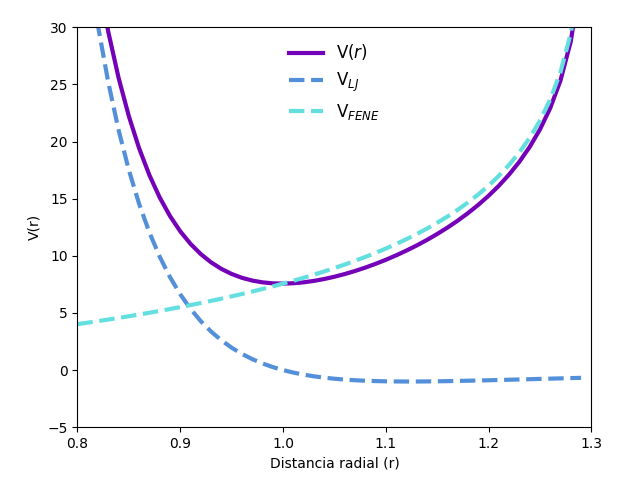
\includegraphics[scale=0.42]{../Graphics/potential.png}
    \caption{Potencial de Lennard-Jones y FENE}
    \label{fig:pot-len-jones}
\end{figure}
\begin{figure}[H]
    \centering
    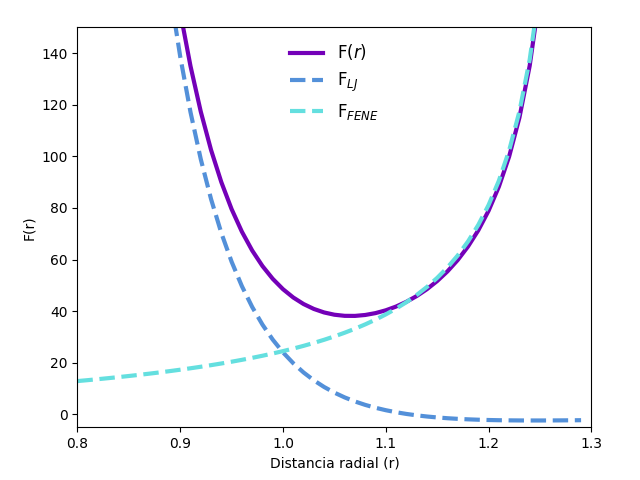
\includegraphics[scale=0.42]{../Graphics/force.png}
    \caption{Fuerza de Lennard-Jones y FENE}
    \label{fig:force-len-jones}
\end{figure}
\begin{table*}
    \centering
    \begin{tabular}{cccccc}
        \hline
        Número de átomos & Número de pasos &$\epsilon_{LJ}$ & $\sigma_{LJ} $ & $K_f$  & R\textsubscript{0} \\ \hline
        \multirow{2}{*}{Variable\textsuperscript{*}} & \multirow{2}{*}{$2x10^{5}$}&\multirow{2}{*}{1} &\multirow{2}{*}{1}  &\multirow{2}{*}{10}   & \multirow{2}{*}{1.3}\\
          & & & & & \\ \hline
    \end{tabular}
    \caption{Parámetros para las diferentes simulaciones del sistema de cadenas de átomos bajo el potencial de Lennard-Jones y el potencial FENE. El número de átomos en cada simulación fueron la siguientes: 100, 200, 300, 400, 500, 600, 700, 800, 900.}
    \label{table:parametros}
\end{table*}
Teniendo definidos los potenciales que actuaran en la simulación
la energía cinética del sistema se estará monitoreando de la siguiente manera:
\begin{equation}
    \label{eq:kin-n}
    T_t=\left\langle \sum_{i=1}^N \frac{1}{2}m|v_i(t)|^2\right\rangle
\end{equation}
por lo tanto, la energía total para un tiempo t será:
\begin{equation}
    \label{eq:e-tot}
    E_t=T_t+U_t
\end{equation}